%\documentclass[aspectratio=43]{beamer}
\documentclass[c]{beamer}
\usetheme{intridea}  %% Themenwahl

\usepackage[ngerman]{babel} 
\usepackage[T1]{fontenc}    % richtige Silbentrennung
\usepackage[utf8]{inputenc} % Umlaute etc.!
\usepackage{eurosym}
\usepackage{tikz}

\usetikzlibrary{arrows,decorations.pathmorphing,backgrounds,fit,positioning,shapes.symbols,chains}

%1

\title{Freifunk Hamburg}
\author{hamburg.freifunk.net}
\date{2013/July/28}


%2
\begin{document}
\maketitle

\begin{frame}{What is freifunk?}
	\begin{itemize}
		\item an initiative for free, cost-free and open, wireless networks
		\item everyone may take part in freifunk as client, provider or both
		\item WiFi routers are access points to the freifunk network
		\item freifunk is available in many places (Berlin, Wien, Augsburg, Lübeck, Kiel, Rheinland, Hamburg...)
	\end{itemize}
\end{frame}


%3
\begin{frame}{What is  freifunk?}
	\textbf{Free} means
	\begin{itemize}
		\item pubic - accessible by everyone
		\item non-commercial
		\item community owned
		\item net neutrality - no manipulation of any data stream
	\end{itemize}
\end{frame}


%4
\begin{frame}{History}
	\begin{itemize}
		\item in the early 2000s the fibre optic network in Berlin-Friedrichshain caused a demand for affordable broadband access
		\item Linksys WRT54g --> Harald Welte gpl-violations.org --> OpenWRT (Jan. 2004)
		\item development of various meshing protocols (OLSR, B.A.T.M.A.N., 802.11s...)
	\end{itemize}
	\begin{center}
		The combination of these three aspects resulted in the demand and the technical prerequesits for freifunk
	\end{center}
\end{frame}


%5
\begin{frame}{How to access the Internet}
	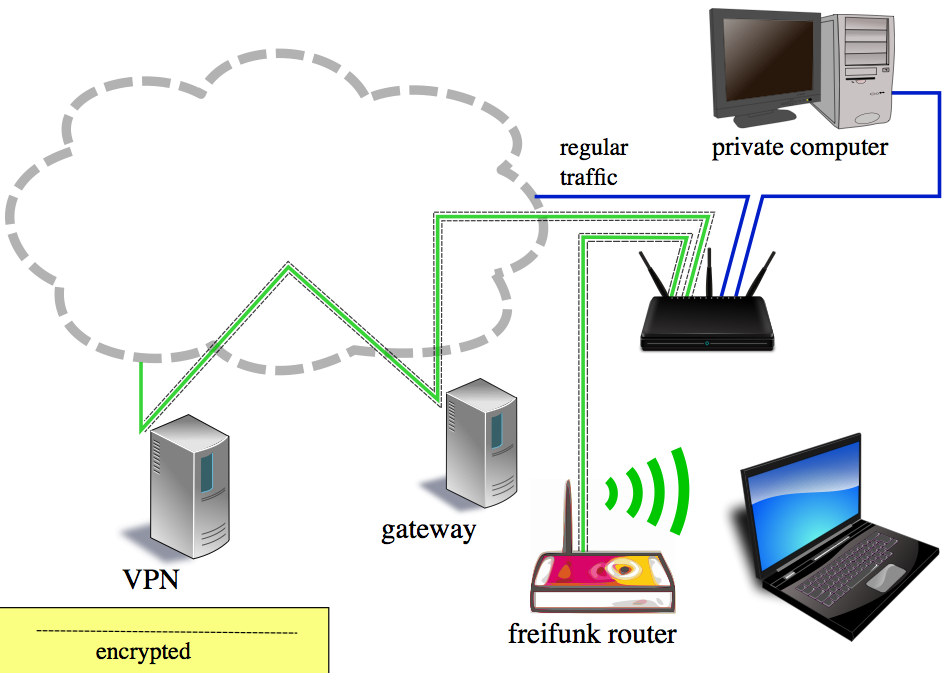
\includegraphics[height=180pt]{Bilder/Knotenanbindung_en}
\end{frame}


%6
\begin{frame}{Project Goals}
	\begin{itemize}
		\item spreading open wireless networks
		\item minimize access barriers to the net
		\item push people's sensitivity on freedom of information
		\item enable people to build their own networks
		\item form and support social structures
	\end{itemize}
\end{frame}


%7
\begin{frame}{Demo}
	\begin{itemize}
		\item node map \href{http://knotenkarte.de/}{http://knotenkarte.de/}
	\end{itemize}
\end{frame}



%8
\begin{frame}{Why WiFi?}
	\begin{itemize}
		\item high data rate mobile solution
		\item hardware and maintenance are reasonably priced (router starting at \EUR{15}, energy for less than \EUR{10} p.a.)
		\item WiFi can be used where no wiring is available / too pricy
	\end{itemize}
\end{frame}


%9
\begin{frame}{Range}
	\begin{center}
		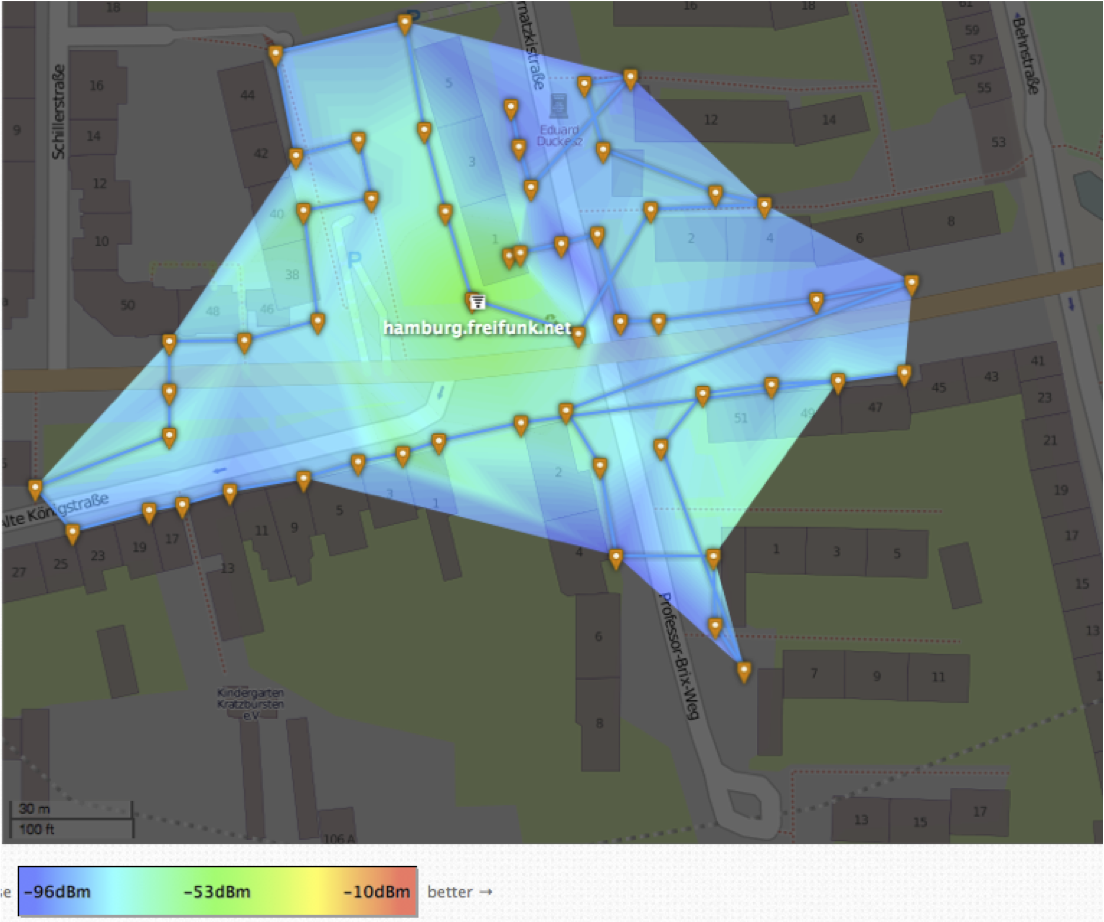
\includegraphics[height=180pt]{Bilder/Reichweite_altona001}
	\end{center}
\end{frame}


%10
\begin{frame}{Mesh}
	What is a mesh?
	\begin{itemize}
		\item self-organizing network
		\item every router is automatically part of the network
		\item hamburg.freifunk.net features the B.A.T.M.A.N.-adv. protocol
	\end{itemize}
	Two SSIDs
	\begin{itemize}
		\item freifunk access: hamburg.freifunk.net
		\item mashing (adhoc): f8:d1:11:87:52:2e
	\end{itemize}
	--> \it Demo [inSSIDer]
\end{frame}


%11
\begin{frame}{Mesh}
	\begin{center}
		\begin{tikzpicture}
			\definecolor{outerCircleColour}{RGB}{220, 0, 103}
			\definecolor{innerCircleColour}{RGB}{255, 203, 18}
			\tikzstyle{vertex}=[circle, draw, color=outerCircleColour, ultra thick, minimum size=84pt]
			\tikzstyle{place}=[circle, draw, color=innerCircleColour, fill=innerCircleColour, minimum size=6pt, inner sep=0pt]

			\node [vertex] (a) {};
			\node [vertex, xshift=68pt, yshift=24pt] (b) {};
			\node [vertex, xshift=112pt, yshift=-20pt] (c) {};

			\node [place, label=above:$A$] (A) {};
			\node [place, xshift=68pt, yshift=24pt, label=above:$B$] (B) {};
			\node [place, xshift=112pt, yshift=-20pt, label=right:$C$] (C) {};

			\path[-, thick, color=gray]
			(A) edge (B)
			(B) edge (C);
		\end{tikzpicture}
	\end{center}
\end{frame}


%12
\begin{frame}{Mesh}
	\begin{center}
		\begin{tikzpicture}
\definecolor{outerCircleColour}{RGB}{220, 0, 103}
			\definecolor{innerCircleColour}{RGB}{255, 203, 18}
			\tikzstyle{vertex}=[circle, draw, color=outerCircleColour, ultra thick, minimum size=84pt]
			\tikzstyle{place}=[circle, draw, color=innerCircleColour, fill=innerCircleColour, minimum size=6pt, inner sep=0pt]

			\node [vertex] (a) {};
			\node [vertex, xshift=68pt, yshift=24pt] (b) {};
			\node [vertex, xshift=112pt, yshift=-20pt] (c) {};

			\node [place, label=above:$A$] (A) {};
			\node [place, xshift=68pt, yshift=24pt, label=above:$B$] (B) {};
			\node [place, xshift=112pt, yshift=-20pt, label=right:$C$] (C) {};

			\path[-, thick, color=gray]
			(A) edge (B)
			(B) edge (C)
			(A) edge[dashed] (C);
		\end{tikzpicture}
	\end{center}
\end{frame}

%13
\begin{frame}{Network Is Growing}
	\begin{center}
		\begin{tikzpicture}
			\definecolor{outerCircleColour}{RGB}{220, 0, 103}
			\definecolor{innerCircleColour}{RGB}{255, 203, 18}
			\tikzstyle{vertex}=[circle, draw, color=outerCircleColour, ultra thick, minimum size=40pt]
			\tikzstyle{place}=[circle, draw, color=innerCircleColour, fill=innerCircleColour, minimum size=7pt, inner sep=0pt]

			\node [vertex] (a) {};
			\node [vertex, xshift=15pt, yshift=30pt] (b) {};
			\node [vertex, xshift=65pt, yshift=5pt] (c) {};
			\node [vertex, xshift=33pt, yshift=-3pt] (d) {};
			\node [vertex, xshift=85pt, yshift=-25pt] (e) {};
			\node [vertex, xshift=100pt, yshift=2pt] (f) {};
			\node [vertex, xshift=91pt, yshift=32pt] (g) {};
			\node [vertex, xshift=110pt, yshift=-52pt] (h) {};
			\node [vertex, xshift=124pt, yshift=23pt] (i) {};
			\node [vertex, xshift=134pt, yshift=-7pt] (j) {};
			\node [vertex, xshift=164pt, yshift=-14pt] (k) {};
			\node [vertex, xshift=144pt, yshift=-66pt] (l) {};
			\node [vertex, xshift=170pt, yshift=-46pt] (m) {};
			\node [vertex, xshift=201pt, yshift=-59pt] (n) {};

			\node [place] (A) {};
			\node [place, xshift=15pt, yshift=30pt] (B) {};
			\node [place, xshift=65pt, yshift=5pt] (C) {};
			\node [place, xshift=33pt, yshift=-3pt] (D) {};
			\node [place, xshift=85pt, yshift=-25pt] (E) {};
			\node [place, xshift=100pt, yshift=2pt] (F) {};
			\node [place, xshift=91pt, yshift=32pt] (G) {};
			\node [place, xshift=110pt, yshift=-52pt] (H) {};
			\node [place, xshift=124pt, yshift=23pt] (I) {};
			\node [place, xshift=134pt, yshift=-7pt] (J) {};
			\node [place, xshift=164pt, yshift=-14pt] (K) {};
			\node [place, xshift=144pt, yshift=-66pt] (L) {};
			\node [place, xshift=170pt, yshift=-46pt] (M) {};
			\node [place, xshift=201pt, yshift=-59pt] (N) {};

			\path[-, thick, color=gray]
			(A) edge (B)
			(A) edge (D)
			(B) edge (D)
			(C) edge (D)
			(C) edge (E)
			(C) edge (F)
			(C) edge (G)
			(E) edge (F)
			(E) edge (H)
			(F) edge (G)
			(F) edge (I)
			(F) edge (J)
			(G) edge (I)
			(H) edge (L)
			(I) edge (J)
			(J) edge (K)
			(K) edge (M)
			(L) edge (M)
			(M) edge (N);
		\end{tikzpicture}
	\end{center}
\end{frame}


%14
\begin{frame}{Networks Are Interconnecting}
	\begin{columns}[c]
		\begin{column}[l]{.4\textwidth}
			\scalebox{0.6}[0.6]{
			\begin{tikzpicture}
				\definecolor{outerCircleColour}{RGB}{220, 0, 103}
				\definecolor{innerCircleColour}{RGB}{255, 203, 18}
				\tikzstyle{vertex}=[circle, draw, color=outerCircleColour, ultra thick, minimum size=40pt]
				\tikzstyle{place}=[circle, draw, color=innerCircleColour, fill=innerCircleColour, minimum size=7pt, inner sep=0pt]

				\node [vertex] (a) {};
				\node [vertex, xshift=15pt, yshift=30pt] (b) {};
				\node [vertex, xshift=65pt, yshift=5pt] (c) {};
				\node [vertex, xshift=33pt, yshift=-3pt] (d) {};
				\node [vertex, xshift=85pt, yshift=-25pt] (e) {};
				\node [vertex, xshift=100pt, yshift=2pt] (f) {};
				\node [vertex, xshift=91pt, yshift=32pt] (g) {};
				\node [vertex, xshift=110pt, yshift=-52pt] (h) {};
				\node [vertex, xshift=124pt, yshift=23pt] (i) {};
				\node [vertex, xshift=134pt, yshift=-7pt] (j) {};
				\node [vertex, xshift=164pt, yshift=-14pt] (k) {};
				\node [vertex, xshift=144pt, yshift=-66pt] (l) {};
				\node [vertex, xshift=170pt, yshift=-46pt] (m) {};
				\node [vertex, xshift=201pt, yshift=-59pt] (n) {};

				\node [place] (A) {};
				\node [place, xshift=15pt, yshift=30pt] (B) {};
				\node [place, xshift=65pt, yshift=5pt] (C) {};
				\node [place, xshift=33pt, yshift=-3pt] (D) {};
				\node [place, xshift=85pt, yshift=-25pt] (E) {};
				\node [place, xshift=100pt, yshift=2pt] (F) {};
				\node [place, xshift=91pt, yshift=32pt] (G) {};
				\node [place, xshift=110pt, yshift=-52pt] (H) {};
				\node [place, xshift=124pt, yshift=23pt] (I) {};
				\node [place, xshift=134pt, yshift=-7pt] (J) {};
				\node [place, xshift=164pt, yshift=-14pt] (K) {};
				\node [place, xshift=144pt, yshift=-66pt] (L) {};
				\node [place, xshift=170pt, yshift=-46pt] (M) {};
				\node [place, xshift=201pt, yshift=-59pt] (N) {};

				\path[-, thick, color=gray]
				(A) edge (B)
				(A) edge (D)
				(B) edge (D)
				(C) edge (D)
				(C) edge (E)
				(C) edge (F)
				(C) edge (G)
				(E) edge (F)
				(E) edge (H)
				(F) edge (G)
				(F) edge (I)
				(F) edge (J)
				(G) edge (I)
				(H) edge (L)
				(I) edge (J)
				(J) edge (K)
				(K) edge (M)
				(L) edge (M)
				(M) edge (N);
			\end{tikzpicture}}
		\end{column}
		\begin{column}{0.185\textwidth}
			\begin{uncoverenv}<2->
				\begin{tikzpicture}
					\definecolor{outerCircleColour}{RGB}{220, 0, 103}
					\definecolor{innerCircleColour}{RGB}{255, 203, 18}

					\draw[color=white] (280pt, 85pt) arc (0:0:0pt);
					\draw[color=white] (-180pt, 85pt) arc (0:0:0pt);

					\draw[color=outerCircleColour, thick, xshift=-50pt, yshift=9pt] (-110pt, 0pt) arc (270:450:6pt);
					\draw[color=outerCircleColour, thick, xshift=-50pt, yshift=11pt] (-110pt, 0pt) arc (270:450:4pt);
					\draw[color=outerCircleColour, thick, xshift=-50pt, yshift=13pt] (-110pt, 0pt) arc (270:450:2pt);

					\draw[color=outerCircleColour, thick, xshift=-9pt, yshift=21pt] (-110pt, 0pt) arc (90:270:6pt);
					\draw[color=outerCircleColour, thick, xshift=-9pt, yshift=19pt] (-110pt, 0pt) arc (90:270:4pt);
					\draw[color=outerCircleColour, thick, xshift=-9pt, yshift=17pt] (-110pt, 0pt) arc (90:270:2pt);

					\draw[color=gray, ultra thick, xshift=-50pt, yshift=15] (-103pt, 0pt) edge[dashed] (-74pt, 0pt);
				\end{tikzpicture}
			\end{uncoverenv}
		\end{column}
		\begin{column}[r]{.5\textwidth}
			\reflectbox{
			\scalebox{0.6}[0.6]{
			\begin{tikzpicture}
				\definecolor{outerCircleColour}{RGB}{220, 0, 103}
				\definecolor{innerCircleColour}{RGB}{255, 203, 18}
				\tikzstyle{vertex}=[circle, draw, color=outerCircleColour, ultra thick, minimum size=40pt]
				\tikzstyle{place}=[circle, draw, color=innerCircleColour, fill=innerCircleColour, minimum size=7pt, inner sep=0pt]

				\node [vertex] (a) {};
				\node [vertex, xshift=15pt, yshift=30pt] (b) {};
				\node [vertex, xshift=65pt, yshift=5pt] (c) {};
				\node [vertex, xshift=33pt, yshift=-3pt] (d) {};
				\node [vertex, xshift=85pt, yshift=-25pt] (e) {};
				\node [vertex, xshift=100pt, yshift=2pt] (f) {};
				\node [vertex, xshift=91pt, yshift=32pt] (g) {};
				\node [vertex, xshift=110pt, yshift=-52pt] (h) {};
				\node [vertex, xshift=124pt, yshift=23pt] (i) {};
				\node [vertex, xshift=134pt, yshift=-7pt] (j) {};
				\node [vertex, xshift=164pt, yshift=-14pt] (k) {};
				\node [vertex, xshift=144pt, yshift=-66pt] (l) {};
				\node [vertex, xshift=170pt, yshift=-46pt] (m) {};
				\node [vertex, xshift=201pt, yshift=-59pt] (n) {};

				\node [place] (A) {};
				\node [place, xshift=15pt, yshift=30pt] (B) {};
				\node [place, xshift=65pt, yshift=5pt] (C) {};
				\node [place, xshift=33pt, yshift=-3pt] (D) {};
				\node [place, xshift=85pt, yshift=-25pt] (E) {};
				\node [place, xshift=100pt, yshift=2pt] (F) {};
				\node [place, xshift=91pt, yshift=32pt] (G) {};
				\node [place, xshift=110pt, yshift=-52pt] (H) {};
				\node [place, xshift=124pt, yshift=23pt] (I) {};
				\node [place, xshift=134pt, yshift=-7pt] (J) {};
				\node [place, xshift=164pt, yshift=-14pt] (K) {};
				\node [place, xshift=144pt, yshift=-66pt] (L) {};
				\node [place, xshift=170pt, yshift=-46pt] (M) {};
				\node [place, xshift=201pt, yshift=-59pt] (N) {};

				\path[-, thick, color=gray]
				(A) edge (B)
				(A) edge (D)
				(B) edge (D)
				(C) edge (D)
				(C) edge (E)
				(C) edge (F)
				(C) edge (G)
				(E) edge (F)
				(E) edge (H)
				(F) edge (G)
				(F) edge (I)
				(F) edge (J)
				(G) edge (I)
				(H) edge (L)
				(I) edge (J)
				(J) edge (K)
				(K) edge (M)
				(L) edge (M)
				(M) edge (N);
			\end{tikzpicture}}}
		\end{column}
	\end{columns}
\end{frame}


%15
\begin{frame}{An Example in Wilhelmsburg}
	\begin{center}
		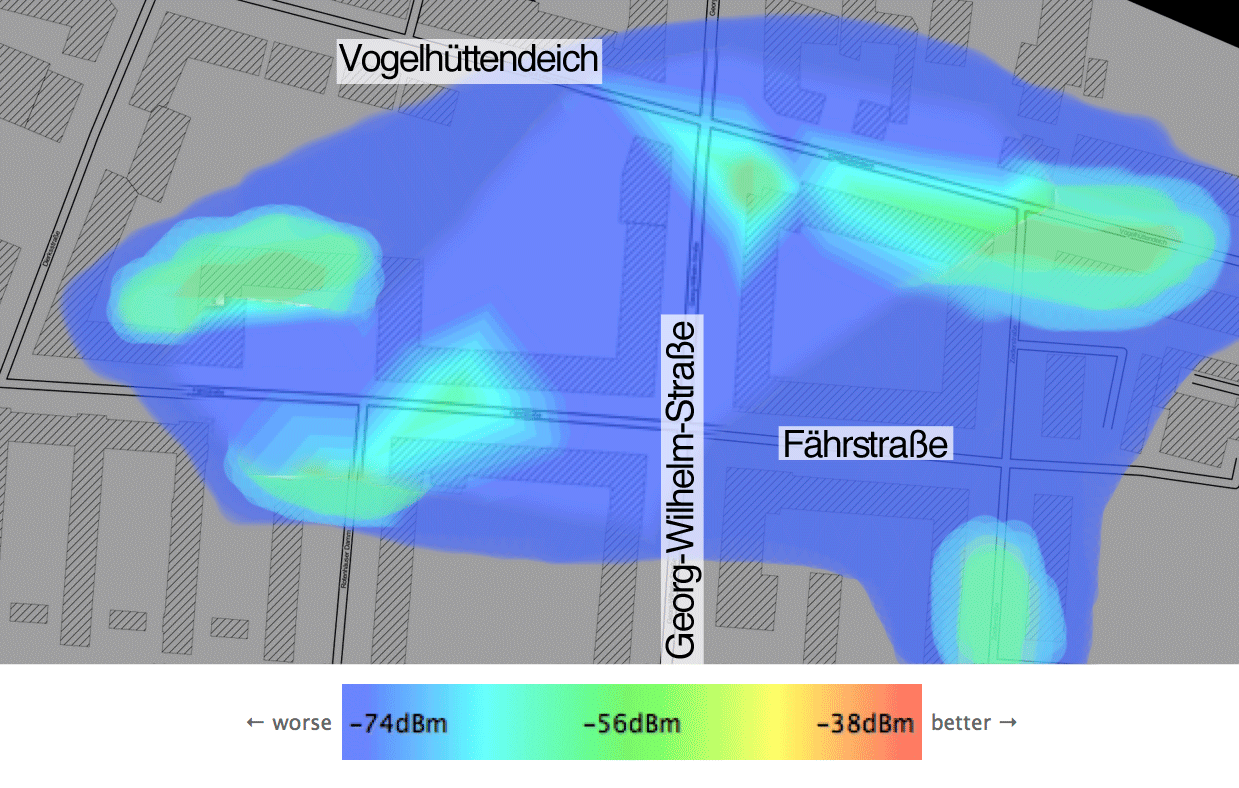
\includegraphics[width=0.9\textwidth]{Bilder/wilhelmsburg}
	\end{center}
\end{frame}


%16
\begin{frame}{Security}
	\begin{itemize}
		\item Since freifunk uses no password, the connection over the air is unencrypted - just like any other open network
		\item It is recommended to make use of encrypted protocols (https://, ftps://, ssh, our your own VPN) – just like anywhere else on the internet
		\item Connections to the gateways are encrypted (fastd) --> no access to the home network possible
	\end{itemize}
\end{frame}


%17
\begin{frame}{Störerhaftung (liability for disturbance)}
	\begin{itemize}
		\item access points do not directly route traffic into the internet
		\item a fastd encrypted connection (VPN) to the gateways is set up over the internet
		\item even the gateways do not directly drop their traffic into the internet, but VPN it abroad
	\end{itemize}
	Consequences:
	\begin{itemize}
		\item \begin{it}Advantage\end{it}: Störerhaftung cannot be enforced
		\item \begin{it}Disadvantage\end{it}: limited bandwith due to encryption effort (ca. 6Mb/s on smaller router models)
	\end{itemize}
\end{frame}


%18
\begin{frame}{Community Agreement}
	\begin{itemize}
		\item be fair!
		\item whatchout for your security!
		\item don't do anything unlawful!
	\end{itemize}
\end{frame}


%19
\begin{frame}{Devices}
	Hardware requirement for Hamburg's freifunk software
	\begin{itemize}
		\item supporting OpenWRT \begin{it}Attitude Adjustment\end{it}
		\item 4 MB flash, 32 MB RAM
		\item It is highly recommended to use routers w/ a current Atheros wireless chip (ath9k-drive, 802.11n-enabled) - they support meshing very well
	\end{itemize}
\end{frame}



%20
\begin{frame}{Devices}
	\begin{columns}[c]
		\begin{column}{0.5\textwidth}
			\begin{itemize}
				\item TP-Link 741nd (starting at \EUR{15})
				\item TP-Link 841nd
				\item TP-Link 842nd (starting at \EUR{25})
				\begin{itemize}
					\item Atheros AR7241 SOC
					\item 8 MB flash	
					\item 32MB RAM
					\item 300Mbit/s
				\end{itemize}
				\item TP-Link 1043nd
				\item TP-Link 3600
			\end{itemize}
		\end{column}
		\begin{column}{0.5\textwidth}
			\begin{center}
				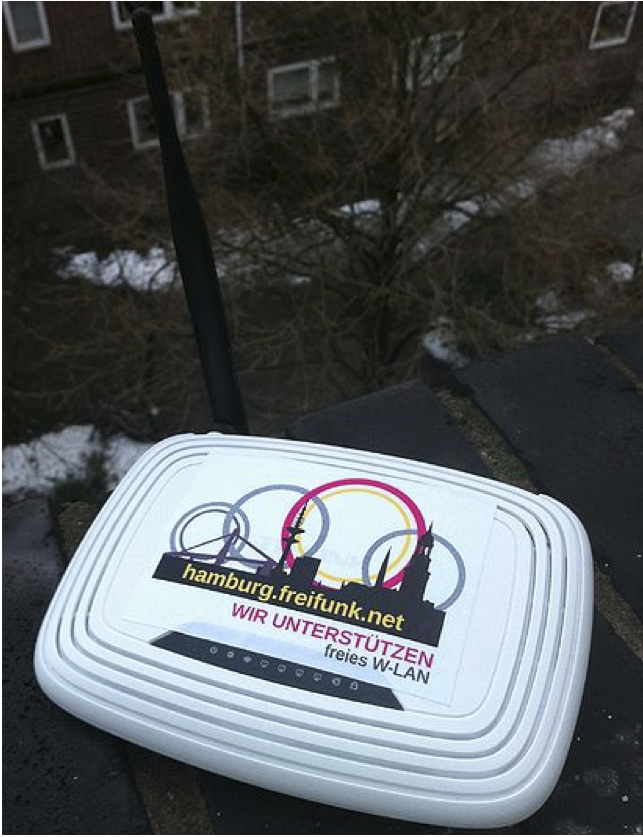
\includegraphics[height=150pt]{741nd}
			\end{center}
		\end{column}
	\end{columns}
\end{frame}


%21
\begin{frame}{Services}
	Implemented
	\begin{itemize}
		\item internet
		\item city-wide intranet (IPv4 \& IPv6)
	\end{itemize}
	Partially Implemented
	\begin{itemize}
		\item IC-VPN, Chaos-VPN, DN42... 
	\end{itemize}
	Yet to Be Implemented
	\begin{itemize}
		\item DNS (for the intranet)
		\item voice over IP (SIP)
		\item anythign else you would like to offer...
	\end{itemize}
\end{frame}


%22
\begin{frame}{Network topology}
	Currently five gateways / DHCP-servers

	Intranet IP ranges
	\begin{itemize}
		\item v4 RFC 1918  range: 10.112.0.0/16
		\item v6 Unique Local Unicast range: fd51:2bb2:fd0d::/48 
	\end{itemize}
	VPN tunnel to \href{https://www.mullvad.net/}{https://www.mullvad.net/}
\end{frame}


%23
\begin{frame}{Demo}
	\begin{itemize}
		\item Checking out / OpenWRT \it Attitude Adjustment
		\item Node statistics at \href{http://www.ohrensessel.net/ffhh/}{http://www.ohrensessel.net/ffhh/}
	\end{itemize}
\end{frame}


%24
\begin{frame}{Outlook}
	\begin{itemize}
		\item increasing number of access points in cafés, restaurants, etc.
		\item cooperations w/ the city of Hamburg (WiFi in parks, tourism...)
		\item cooperation w/ public transportation (HVV)
		\item universities, student union
		\item ...
	\end{itemize}
\end{frame}


%25
\begin{frame}{Projects}
	\begin{itemize}
		\item customizing antennas
		\item outdoor housings
		\item solar-powered routers
		\item flash workshops
		\item PPPoE
		\item private wireless network
		\item uplink over wireless
		\item remote monitoring and updates of nodes
		\item setting up a mail server on srv01
		\item form to alter your own router settings in the DB
		\item ...
	\end{itemize}
\end{frame}


%26
\begin{frame}{How Can I Participate?}
	\begin{itemize}
		\item freifunk is open to everyone - no technical expertise required
		\item become part of the network by setting up a router
		\item meet up Monday's at 19:00 at the CCCHH
		\item promote the idea!
	\end{itemize}
\end{frame}


%27
\begin{frame}{Thatks for Your Attention!}
	\begin{columns}
		\begin{column}{0.6\textwidth}
			\begin{itemize}
				\item web hamburg.freifunk.net
				\item mail: kontakt@hamburg.freifunk.net
		\end{itemize}
		\end{column}
		\begin{column}{0.5\textwidth}
			\begin{center}
				
\includegraphics[width=0.5\textwidth]{Bilder/cc-by}
			\end{center}
		\end{column}
	\end{columns}
\end{frame}

\end{document}